\section{Nombre: Plataforma que cae.}\label{obs.plataformaD}
	\subsection{Descripción}
	Porción de suelo que cae después de n cantidad de segundos que el jugador ha aterrizado sobre ella.
	\subsection{Esquema}
Ver figura \ref{fig:PlatCae}.
	\begin{figure}
  \centering
  \subfigure[El jugador aterriza sobre la plataforma que cae.]{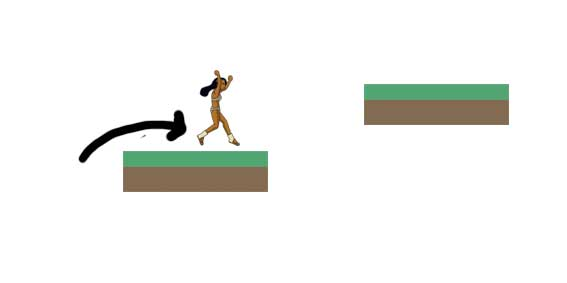
\includegraphics[width=0.5 \textwidth]{Imagenes/platCae01}}
   \subfigure[La plataforma cae después de n cantidad de tiempo.]{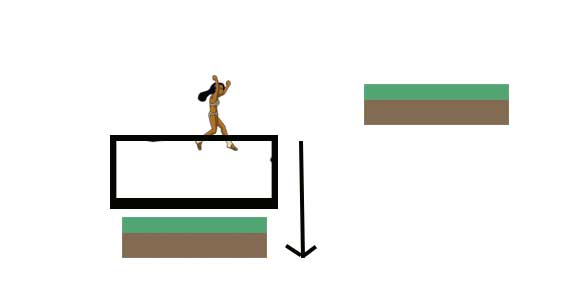
\includegraphics[width=0.5 \textwidth]{Imagenes/platCae02}}
  \caption{Plataforma que cae.}
  \label{fig:PlatCae}
\end{figure} 